\documentclass[tikz,border=7pt]{standalone}
% Shared visual language for the book's standalone vector figures.
% Keep this file compatible with the TeX Live version used by LyX.
\usepackage{amsmath,amssymb}
\usepackage{array,booktabs}
\usepackage{pgfplots}
\usepackage{pgfplotstable}
\usetikzlibrary{arrows.meta,calc,positioning}
\pgfplotsset{compat=1.17}

\definecolor{BookBlue}{HTML}{0072B2}
\definecolor{BookOrange}{HTML}{D55E00}
\definecolor{BookGreen}{HTML}{009E73}
\definecolor{BookGray}{HTML}{666666}
\definecolor{BookLightGray}{HTML}{D9D9D9}

\pgfplotsset{
  book axis/.style={
    axis line style={black!75,line width=0.55pt},
    tick style={black!75,line width=0.45pt},
    tick label style={font=\small},
    label style={font=\small},
    legend style={
      font=\small,
      draw=none,
      fill=none,
      cells={anchor=west},
    },
    grid style={BookLightGray,line width=0.35pt},
    major grid style={BookLightGray,line width=0.35pt},
  },
}

\begin{document}
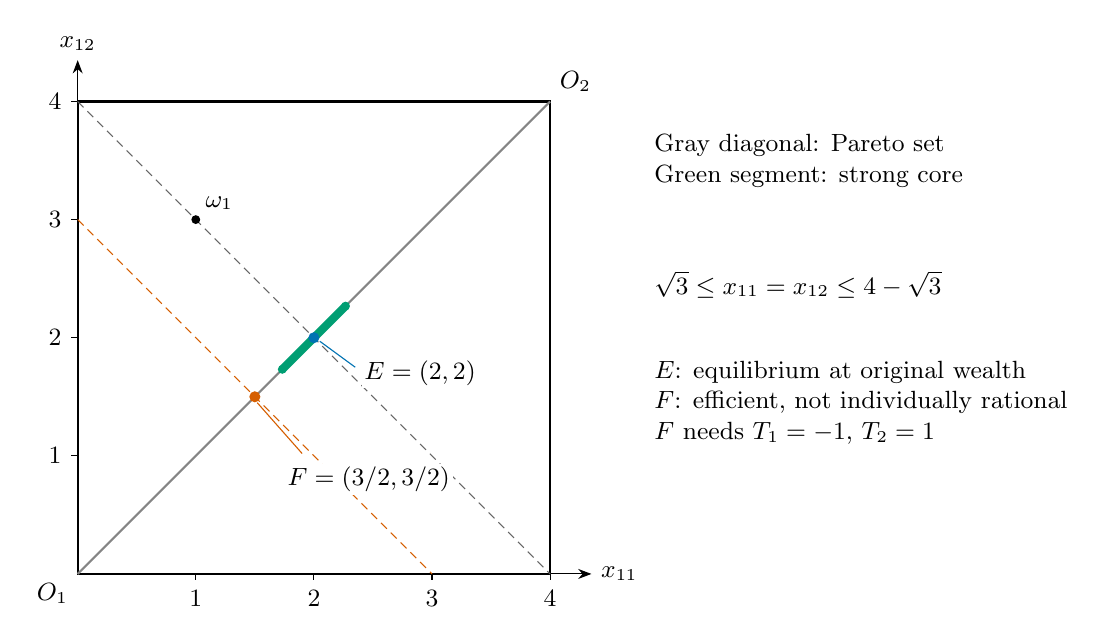
\begin{tikzpicture}[x=1.5cm,y=1.5cm,>=Stealth,font=\small]
  \draw[thick] (0,0) rectangle (4,4);
  \draw[->] (0,0)--(4.35,0) node[right] {$x_{11}$};
  \draw[->] (0,0)--(0,4.35) node[above] {$x_{12}$};
  \node[below left] at (0,0) {$O_1$};
  \node[above right] at (4,4) {$O_2$};
  \foreach \v in {1,2,3,4} {
    \draw (\v,0)--(\v,-.055) node[below] {$\v$};
    \draw (0,\v)--(-.055,\v) node[left] {$\v$};
  }
  \draw[BookGray!80,thick] (0,0)--(4,4);
  \draw[BookGreen,line width=3pt] ({sqrt(3)},{sqrt(3)})--({4-sqrt(3)},{4-sqrt(3)});
  \fill[BookGreen] ({sqrt(3)},{sqrt(3)}) circle(1.6pt);
  \fill[BookGreen] ({4-sqrt(3)},{4-sqrt(3)}) circle(1.6pt);
  \draw[BookGray,densely dashed] (0,4)--(4,0);
  \draw[BookOrange,densely dashed] (0,3)--(3,0);
  \fill (1,3) circle(1.6pt) node[above right] {$\omega_1$};
  \fill[BookBlue] (2,2) circle(2pt);
  \node[anchor=west,fill=white,inner sep=1pt] at (2.4,1.7) {$E=(2,2)$};
  \draw[BookBlue] (2.05,1.97)--(2.35,1.75);
  \fill[BookOrange] (1.5,1.5) circle(2pt);
  \node[anchor=west,fill=white,inner sep=1pt] at (1.75,.8) {$F=(3/2,3/2)$};
  \draw[BookOrange] (1.52,1.45)--(1.9,1.02);
  \node[anchor=west,align=left] at (4.8,3.5) {Gray diagonal: Pareto set\\Green segment: strong core};
  \node[anchor=west,align=left] at (4.8,2.45) {$\sqrt3\leq x_{11}=x_{12}\leq4-\sqrt3$};
  \node[anchor=west,align=left] at (4.8,1.45) {$E$: equilibrium at original wealth\\$F$: efficient, not individually rational\\$F$ needs $T_1=-1$, $T_2=1$};
\end{tikzpicture}
\end{document}
